\documentclass{article}
\usepackage[T1]{fontenc}
\usepackage[utf8]{inputenc}
\usepackage{hyperref}
\usepackage{graphicx}
\usepackage{caption}
\usepackage{subcaption}
\usepackage{array}
\usepackage{geometry}
\usepackage{amsfonts}
\usepackage{booktabs}
\usepackage{multirow}

\title{Parallel programming for HPC: exam project\\ Exercise 3: MPI one-sided communication for the Jacobi method}
\author{\textbf{Student:} Isac Pasianotto}
\date{2024-06}

\setcounter{section}{-1} % Start section numbering from 0
\renewcommand{\thesection}{\arabic{section}} % Adjust section numbering in the table of contents

\begin{document}
    \maketitle
    %\tableofcontents

    \section{Requirements}

    The task this assignment aims  to solve is the parallelization of the Jacobi method using MPI one-sided communication.
    The starting point is the already parallelized version of the Jacobi method using MPI point-to-point communication, which is the solution of the previous exercise.

   \section{Implementation}

    Since the focus of this exercise is the communication between processes, all the section of the code responsible for the GPU computation has been removed, and
    the faster version of the output savin (MPI I/O) has been used.

    The amount of data to be exchanged between processes is the same as in the previous exercise, but the communication is done using remote memory access (RMA) operations.

    Since no specification was given about how precisely this communication should be performed, the following case has been implemented:

    \begin{table}[h]
        \centering
        \begin{tabular}{@{}lcc@{}}
                                              & \multicolumn{2}{c}{Operation used to retrieve Data} \\ \cmidrule(l){2-3}
          \multirow{2}{*}{Number of windows}  & 1 Window - PUT            & 1 Window - GET            \\ \cmidrule(l){2-3}
                                              & 2 Windows - PUT           & 2 Windows - PUT           \\
        \end{tabular}
        \caption{Different implementations of RMA}
    \end{table}

    With 1 window, I mean that the process will open a \texttt{MPI\_Win} object exposing to other processes the whole matrix, while with 2 windows, the process will open two \texttt{MPI\_Win} objects, one for the first row and one for the last row of the matrix.
    The notation PUT and GET should be self-explanatory: the first one is used to write data to the remote process with \texttt{MPI\_Put}, while the second one is used to read data from the remote process with \texttt{MPI\_Get}.

    \section{Results}

    To keep consistency with the previous exercises, the code has been run for two different matrix sizes and a fixed number of iterations:

    \begin{itemize}
        \itemsep0em
        \item \textit{Matrix size:} $1,200 \times 1,200$, \textit{Iterations:} $10$
        \item \textit{Matrix size:} $12,000 \times 12,000$, \textit{Iterations:} $10$
    \end{itemize}

    The code was run on the \href{https://leonardo-supercomputer.cineca.eu/}{Leonardo} cluster on \href{https://wiki.u-gov.it/confluence/display/SCAIUS/UG3.2.2%3A+LEONARDO+DCGP+UserGuide}{DCGP} nodes, which are used for CPU computing, spawning one MPI process per node, and let OpenMP use all the available cores in the node.

    The results are represented in the plots in the following pages, but can be summarized as follows:

    \begin{itemize}
        \itemsep0em
       \item \texttt{MPI\_Get} function seems to perform a little better than \texttt{MPI\_Put}. However, this difference becames less evident scaling up the number of nodes and the matrix size
        \item The communication time of the one and two windows cases seems to be almost the same. The initialization time required to open the window is less in the one-window case
        \item The \texttt{RMA} approach seems to have a faster communication compared with \texttt{MPI\_Send} + \texttt{MPI\_Recv}. But the initialization time obliterates this advantages.
        \item Probably for a higher number of iteration RMA can be the best choice.
    \end{itemize}

    \newpage

    \subsection{\texttt{MPI\_Put} vs \texttt{MPI\_Get}}

    \begin{figure}
        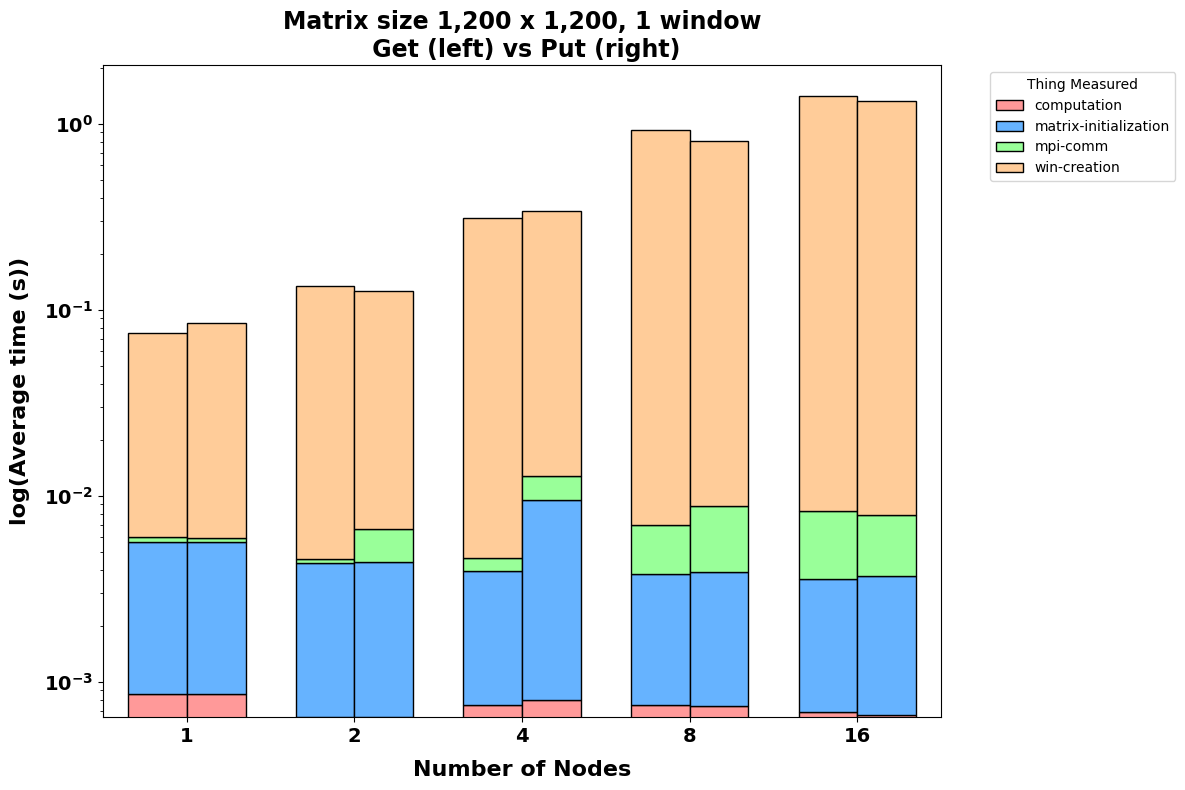
\includegraphics[width=\textwidth]{./images/getvsput-1win-1200}
        \caption{Matrix size: $1,200 \times 1,200$, 1 \texttt{MPI\_Win}.}
        \label{fig:figure1}
    \end{figure}

    \begin{figure}
        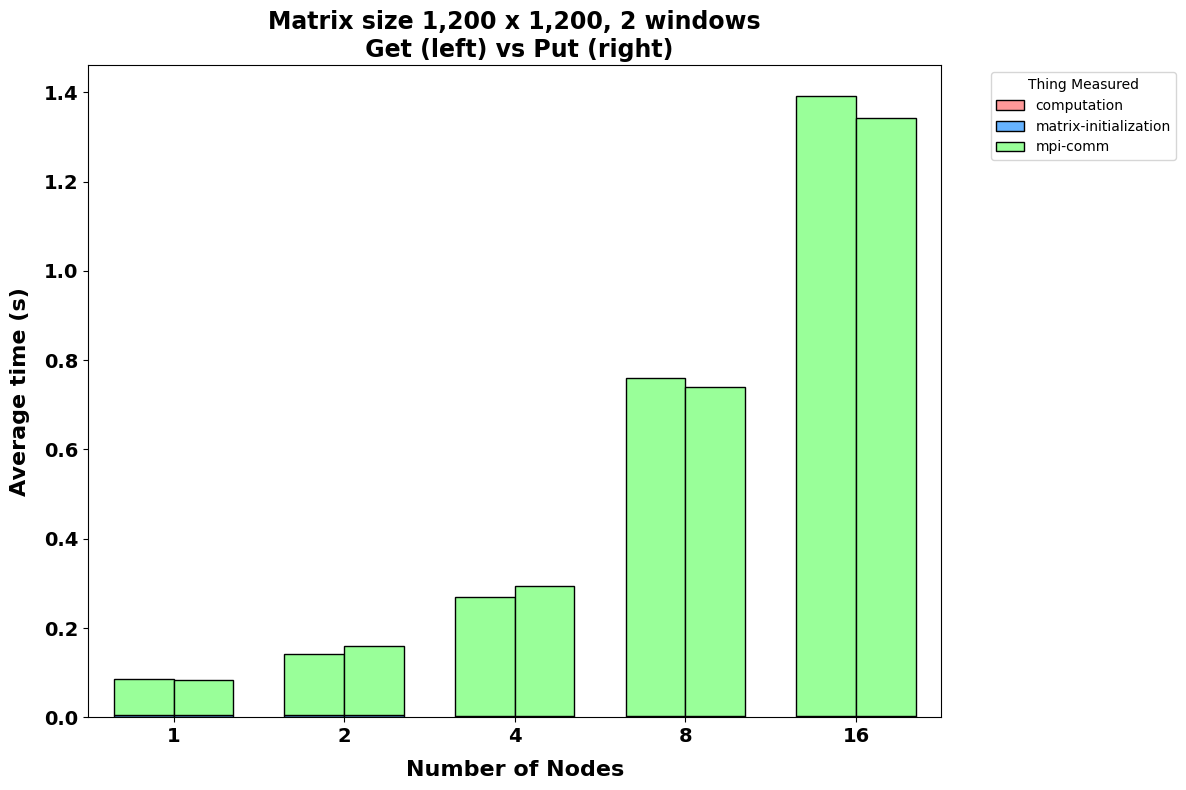
\includegraphics[width=\textwidth]{./images/getvsput-2win-1200}
        \caption{Matrix size: $1,200 \times 1,200$, 2 \texttt{MPI\_Win}.}
        \label{fig:figure2}
    \end{figure}


    \begin{figure}
        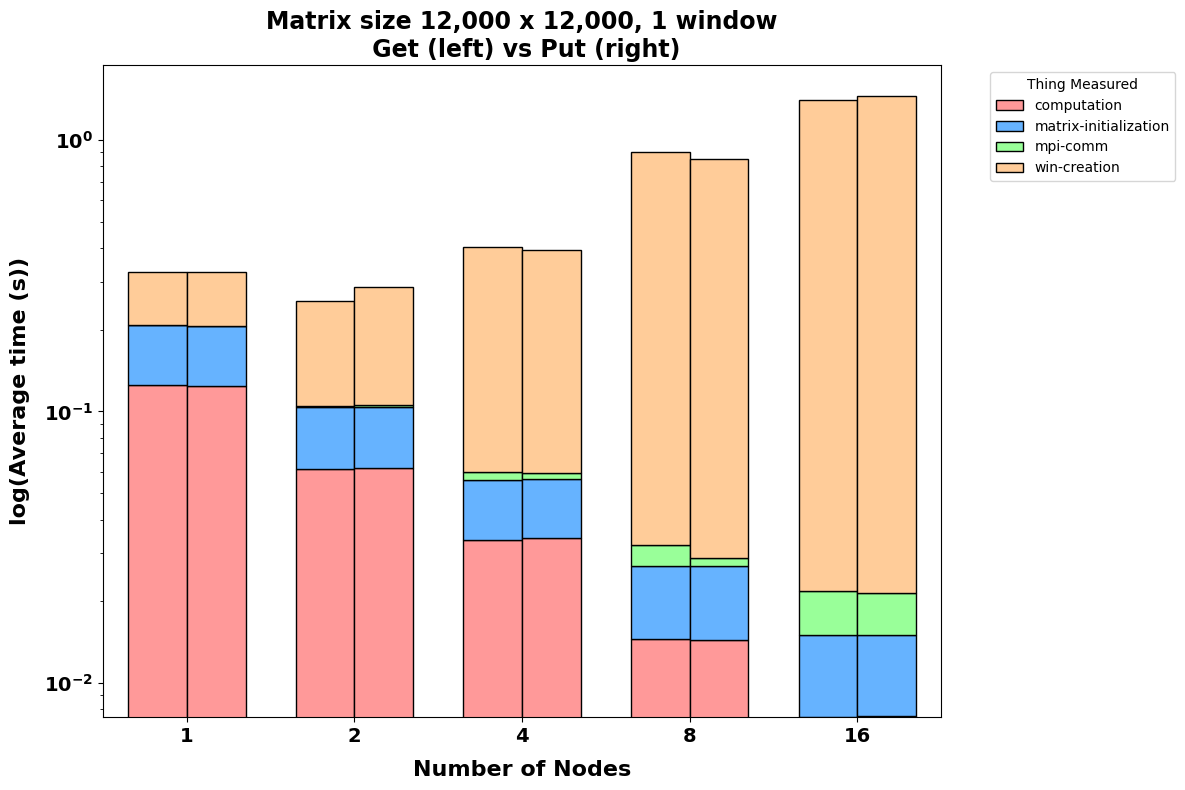
\includegraphics[width=\textwidth]{./images/getvsput-1win-12k}
        \caption{Matrix size: $12,000 \times 12,000$, 1 \texttt{MPI\_Win}.}
        \label{fig:figure3}
    \end{figure}

    \begin{figure}
        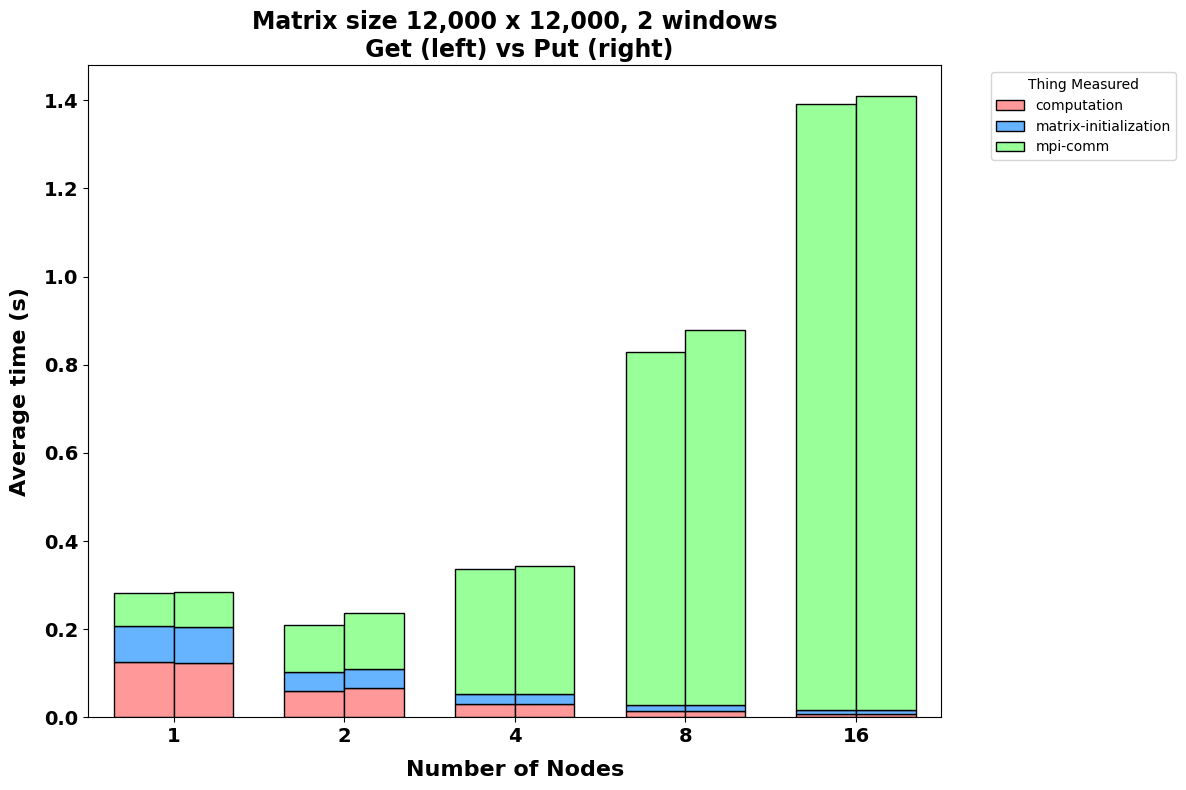
\includegraphics[width=\textwidth]{./images/getvsput-2win-12k}
        \caption{Matrix size: $12,000 \times 12,000$, 2 \texttt{MPI\_Win}.}
        \label{fig:figure4}
    \end{figure}

    \newpage
    \subsection{1 window vs 2 windows}

    For the following plots, the \texttt{MPI\_Put} function has been chosen as the communication method.

    \noindent Moreover, to have a comparison with the previous exercise, the results of the MPI point-to-point communication have been included, using \texttt{MPI\_Isend} and \texttt{MPI\_Irecv} functions.


    \begin{figure}
        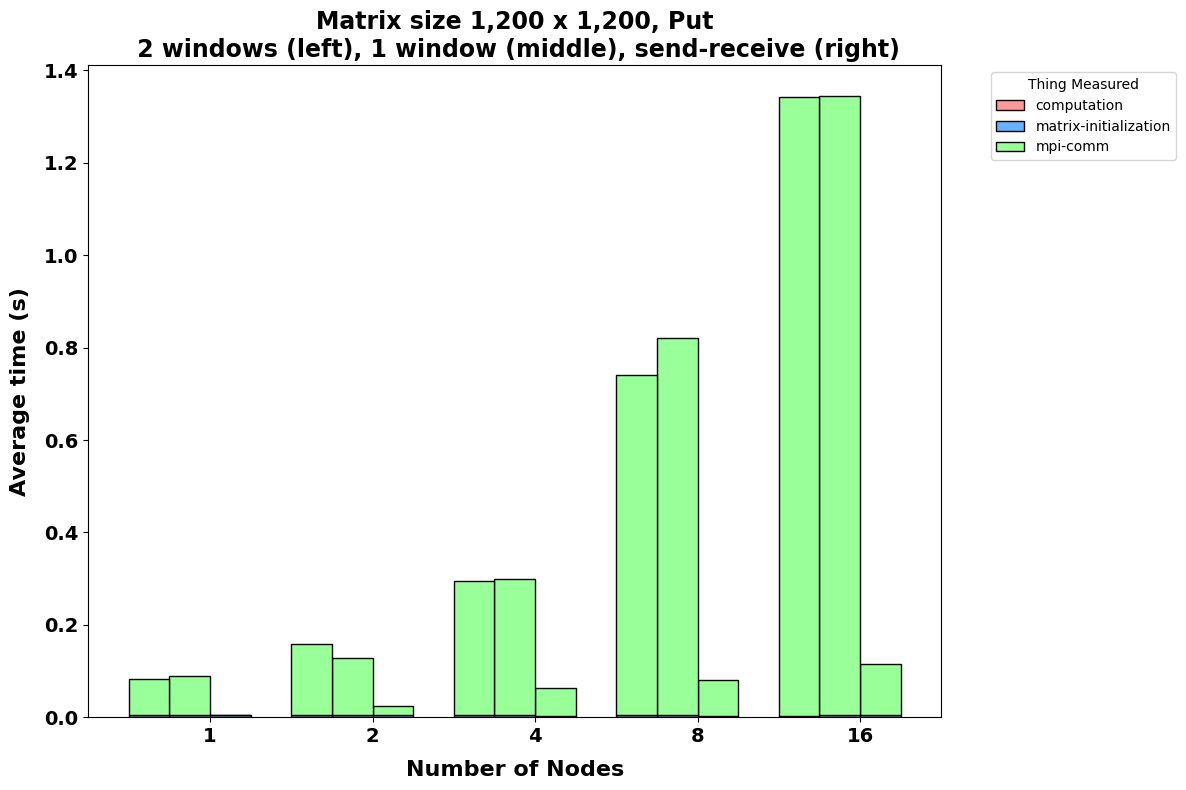
\includegraphics[width=\textwidth]{./images/1winvs2win-1200}
        \caption{Matrix size: $1,200 \times 1,200$. The performance of the 1 window and 2 windows implementations is very similar.}
        \label{fig:figure5}
    \end{figure}

    \begin{figure}
        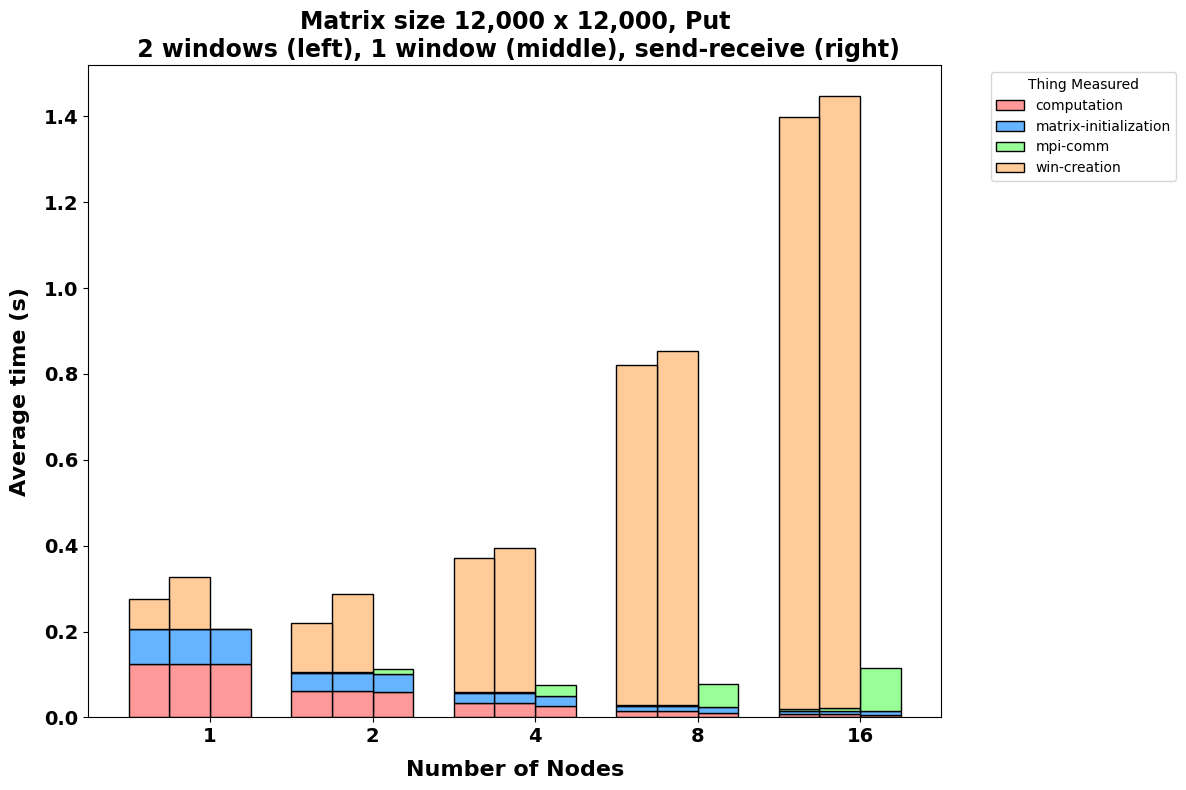
\includegraphics[width=\textwidth]{./images/1winvs2win-12k}
        \caption{Matrix size: $12,000 \times 12,000$.}
        \label{fig:figure6}
    \end{figure}

\end{document}
